\documentclass[letterpaper,twocolumn,10pt]{article}
\usepackage{usenix2019_v3}

\usepackage{amsmath,amssymb}
\usepackage{graphicx}
\usepackage{booktabs}
\usepackage{multirow}
\usepackage[binary-units]{siunitx}
\usepackage{tikz}
\usetikzlibrary{arrows.meta,positioning}
\usepackage{pifont}
\usepackage{algorithm}
\usepackage{algpseudocode}
\usepackage{enumitem}
\usepackage{listings}
\usepackage{xcolor}

\sisetup{detect-weight=true, detect-family=true}

\graphicspath{{../results/latest/figures/}{figures/}}

\date{}

\title{\Large \bf GAIA: GPU Microarchitectural Power Attacks\\and Countermeasures for AI Data Centers}
\author{{\rm Anonymous submission \#XXX to USENIX Security '27}\\
Do not distribute.}

\begin{document}
\maketitle

% ===================================================================
\begin{abstract}
AI data centers concentrate high-power GPUs behind shared power
distribution networks, creating attack surfaces absent from
traditional multi-tenant environments.
We present GAIA, the first systematic study of GPU
microarchitectural power attacks on AI infrastructure.
On an NVIDIA Jetson AGX Thor (Blackwell, 130\,W TDP), six
adversarial primitives---cache-eviction, compute saturation,
10\,kHz pulsed modulation, occupancy flooding,
temperature-synchronized stress, and sustained combined
stress---are evaluated across 10 randomized trials with three
victim workload types.
Sustained stress elevates power to $1.83\times$ baseline (peak
81.1\% TDP) with workload-dependent latency impact:
$+$92\% (matmul), $+$32\% (CNN training), $+$4\% (inference).
A logistic regression classifier over eight telemetry features
achieves 96.9\% accuracy (ROC-AUC = 0.9816, LOTO-CV); FFT
spectral analysis shows 1.4--53.7$\times$ energy separation
($p{=}0.016$); PCA confirms three components (81.7\% variance)
cleanly separate attack from baseline.
A power-budget sweep shows oversubscription persists at every
clock cap ($+$16\,W to $+$43\,W), and matched-load contention
isolation reveals $+$16.1\% excess degradation from power-domain
interference alone.
Two mitigation strategies exhibit workload-dependent tradeoffs:
clock capping (18--24\% power reduction, up to $+$74.5\% victim
latency cost) versus graceful termination (41--43\% recovery,
5--6\% latency overhead).  Blinded adversary attribution via
baseline-recovery scoring achieves 100\% accuracy (5/5 trials),
completing an end-to-end attack--detect--attribute--mitigate pipeline
with Prometheus-compatible telemetry.
\end{abstract}

% ===================================================================
\section{Introduction}
\label{sec:intro}
% ===================================================================

Hyper-specialized GPU data centers have become the cornerstone of the
modern AI revolution.  The Northern Virginia region alone hosts the
world's highest concentration of data centers~\cite{eia2026}, and
utilities such as Dominion Energy are preparing for $3\times$ their
current peak load to accommodate GPU-centric
infrastructure~\cite{jlarc2024,dominion2026}.  This concentration creates a
critical vulnerability: coordinated power manipulation on AI data
center hardware may propagate across the power grid under adversarial
conditions~\cite{choukse2025}.  Recent collaborative work by
Microsoft, OpenAI, and NVIDIA has demonstrated that harmonized power
swings from large training workloads can physically damage grid
infrastructure~\cite{watchus2025,semieng2025}, establishing that
power-domain threats to AI infrastructure are not hypothetical.

Prior work has examined power attacks against traditional multi-tenant
data centers (MTDCs).  Islam et al.~\cite{islam2017} demonstrated
that co-located tenants can induce measurable power fluctuations, and
subsequent work showed voltage side channels exploitable for timing
attacks~\cite{islam2018}.  Xu et al.~\cite{xu2014} characterized
power attacks as an increasing threat to data center availability.
However, GPU-based AI training facilities have distinct power,
memory, and computational load profiles compared to traditional
CPU-based compute servers; modern GPUs can draw hundreds of watts
per device, share power delivery infrastructure across compute
domains, and exhibit workload-dependent power phases that create
new attack surfaces.

Despite this growing threat landscape, \emph{no prior work has
systematically investigated GPU microarchitectural power attacks on
AI data center hardware.}  Existing GPU security research has
focused on cache side channels, rowhammer-style fault injection,
and information leakage---but not on the power domain as an attack
vector.  Wang et al.~\cite{wang2025} recently demonstrated that GPU
cache-eviction priority hints have significant security implications,
and Yandrofski et al.~\cite{yandrofski2022} showed that adversarial
CUDA kernels can disrupt real-time system guarantees, but neither
work addresses the power-domain attack surface that AI data centers
uniquely expose.

This gap motivates a fundamental research question: \emph{How can
power attacks on GPU hardware in modern AI data centers be designed,
evaluated, detected, and mitigated to prevent infrastructure
disruptions?}

We address this question with Project GAIA (\textbf{G}PU
\textbf{A}ttack \textbf{I}nvestigation and \textbf{A}nalysis),
structured around three research thrusts:

\begin{itemize}[nosep]
\item \textbf{Thrust~1 (Attack Design):} Design benign-looking
  microarchitectural workloads that force co-located training
  applications to draw more power, driving multi-tenant GPU servers
  toward oversubscription and system instability.
\item \textbf{Thrust~2 (Detection):} Develop and evaluate defense
  mechanisms for detecting power attacks using GPU hardware telemetry
  and power services.
\item \textbf{Thrust~3 (Mitigation):} Prototype an end-to-end
  closed-loop monitoring pipeline to flag anomalous power-driven
  load and apply real-time mitigation.
\end{itemize}

Our experiments are conducted on an NVIDIA Jetson AGX Thor developer
kit (Blackwell architecture, sm\_110, 130\,W TDP) using hardware
power sensors (INA3221 via sysfs) and GPU telemetry (devfreq, thermal
zones).  We evaluate attack impact across three victim workload
types---synthetic matrix multiply, CNN training, and CNN inference---to
characterize workload-dependent attack effectiveness, a phenomenon
that emerges as the central finding of this work.

Our contributions are:

\begin{enumerate}[nosep]
\item \textbf{First systematic GPU power attack characterization.}
  We design and evaluate six adversarial workload primitives that
  exploit GPU microarchitectural features (L2 cache hints, compute
  saturation, clock-domain interactions) to manipulate server power
  draw, and demonstrate workload-dependent attack effectiveness
  across three victim types.

\item \textbf{Honest detection evaluation with failure analysis.}
  We evaluate threshold and ML-based detectors and report per-condition
  performance breakdowns that reveal a 44.4\% FPR on legitimate
  high-power workloads---demonstrating that power-level features
  alone are insufficient for production deployment.

\item \textbf{Workload-aware mitigation with decomposition analysis.}
  We demonstrate that clock capping and process termination have
  workload-dependent tradeoffs, and provide a formal decomposition
  separating clamping overhead from net attack effects.

\item \textbf{Complete attack--detect--mitigate pipeline.}
  We integrate all three thrusts into a closed-loop system with
  Prometheus-compatible telemetry, demonstrating end-to-end feasibility.
\end{enumerate}


% ===================================================================
\section{Background and Threat Model}
\label{sec:background}
% ===================================================================

\subsection{GPU Power Delivery Architecture}
\label{sec:bg-power}

Modern data center GPUs consume 300--700\,W per device, supplied
through multi-phase voltage regulator modules (VRMs) that convert
a 12\,V or 48\,V rack-level supply into the sub-1\,V core voltages
required by GPU die domains.  Power delivery networks (PDNs) in GPU
servers are designed for the thermal design power (TDP) of each
device, with limited headroom for sustained over-TDP transients.

In AI training clusters, power consumption is bursty and
synchronized: the dominant training paradigm (data-parallel SGD)
causes all GPUs in a training job to execute the same computational
phases simultaneously.  Choukse et al.~\cite{choukse2025}
demonstrated that these synchronized power phases can create
aggregate power swings of hundreds of kilowatts at the facility
level, sufficient to interact with power distribution equipment.

The Jetson AGX Thor used in our experiments provides a
single-board analog of this architecture: the module-level INA3221
sensor monitors total board power (including GPU, CPU/SoC, I/O,
and memory domains) from a shared $\sim$19.74\,V supply rail.
While the integrated GPU's power delivery differs from discrete
data center GPUs (which have independent power planes and support
\texttt{nvidia-smi --power-limit}), the shared-rail architecture
is directly relevant to the threat model: adversarial kernels on
one compute domain affect power draw on the shared rail, impacting
co-located workloads.

\subsection{GPU Microarchitecture Relevant to Attacks}
\label{sec:bg-uarch}

Three GPU microarchitectural features are central to our attack
design:

\textbf{L2 cache and memory hierarchy.}
NVIDIA GPUs expose cache-control hints through PTX instructions.
The \texttt{st.global.wt} (write-through) and \texttt{ld.global.cg}
(cache-global, evict-first) instructions bypass or evict L2 cache
lines, forcing repeated DRAM accesses that draw significantly more
power than cache-serviced operations.  Wang et al.~\cite{wang2025}
demonstrated that these cache-eviction priority hints have
measurable security and performance implications.

\textbf{Streaming Multiprocessors (SMs) and occupancy.}
Each SM can host a hardware-limited number of concurrent warps.
An adversary that launches kernels with minimal per-thread resources
(registers, shared memory) can maximize warp occupancy, consuming
SM scheduling slots and power budget while starving co-located
victims of execution resources.

\textbf{Dynamic Voltage and Frequency Scaling (DVFS).}
GPUs dynamically adjust clock frequency based on power, thermal, and
utilization conditions via the devfreq governor.  This creates a
bidirectional interaction: adversarial load raises the power floor,
potentially triggering thermal throttling, while DVFS responses
(clock changes) affect both attacker and victim performance.  Our
mitigation exploits this same mechanism by externally capping the
clock frequency.

\subsection{Threat Model}
\label{sec:threat}

We assume a malicious or compromised tenant with \emph{user-level}
access co-located on a multi-tenant GPU training server.  The
attacker's goal is to manipulate the temporal power profile of the
shared server where benign AI training jobs are running.  The
attacker:

\begin{itemize}[nosep]
\item Has standard CUDA user-space access (can launch kernels, use
  PTX inline assembly).
\item Has \emph{no} root, firmware, physical, or facility-level
  power-system access.
\item Cannot access other tenants' memory or processes.
\item Can observe public GPU state: temperature via sysfs thermal
  zones, clock frequency via devfreq.
\end{itemize}

The adversary's objectives include: (1)~elevating aggregate server
power toward or beyond the provisioned capacity, potentially
triggering infrastructure-level protections (circuit breakers,
UPS failover); (2)~degrading co-located victim workload performance
through power-domain contention; and (3)~creating periodic power
oscillations that could interact with PDN resonances at facility
scale.

\textbf{Scope and limitations.}  Our experiments are conducted on a
single Jetson AGX Thor developer kit, not a multi-GPU data center
server.  We measure local power-domain effects (power elevation,
victim degradation, detection feasibility) as proxies for the
data-center-scale threat.  We do not claim that single-GPU power
manipulation directly causes grid instability; rather, we establish
the per-device attack surface that would be amplified in a
multi-GPU, multi-rack deployment.

% Project GAIA — Threat Model & Defense Pipeline (TikZ)
% IEEEtran conference double-column figure
\begin{figure*}[t]
\centering
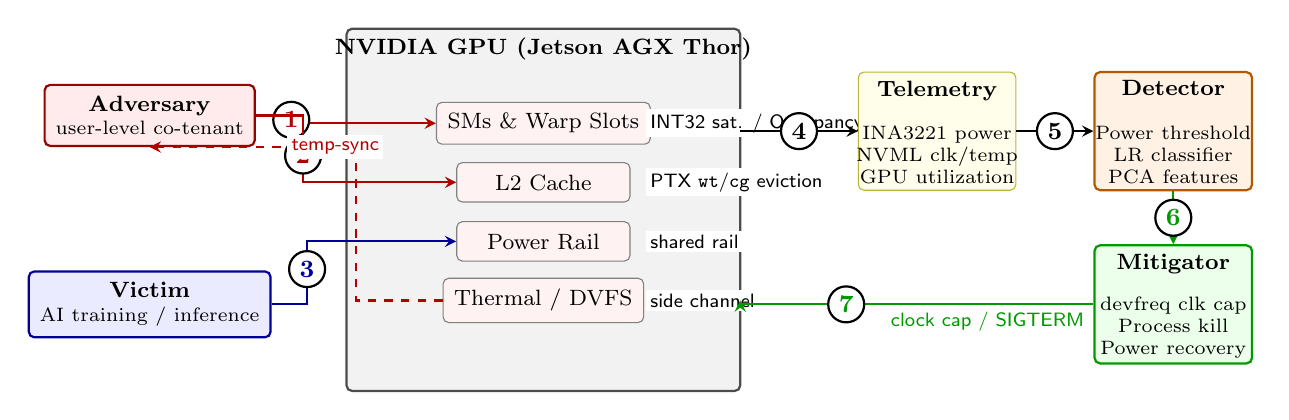
\begin{tikzpicture}[
    >=stealth,
    every node/.style={font=\footnotesize},
    box/.style={draw, rounded corners=2pt, minimum height=0.65cm,
                align=center, fill=#1, inner sep=4pt},
    box/.default=white,
    attackbox/.style={box=red!8, draw=red!60!black, thick},
    victimbox/.style={box=blue!8, draw=blue!60!black, thick},
    gpubox/.style={box=gray!10, draw=black!70, thick},
    detectbox/.style={box=orange!10, draw=orange!70!black, thick},
    mitigatebox/.style={box=green!8, draw=green!60!black, thick},
    telbox/.style={box=yellow!8, draw=yellow!70!black},
    resbox/.style={box=red!5, draw=gray, minimum width=2.2cm, minimum height=0.5cm},
    lbl/.style={font=\scriptsize\sffamily, fill=white, inner sep=1.5pt},
    cnum/.style={circle, draw=black, fill=white, font=\scriptsize\bfseries,
                 inner sep=0.5pt, minimum size=13pt},
    arr/.style={->, thick},
    darr/.style={->, thick, dashed},
]

% ===== LEFT: ACTORS =====
\node[attackbox, minimum width=2.2cm] at (0, 1.2)
    (attacker) {\textbf{Adversary}\\[-1pt]{\scriptsize user-level co-tenant}};

\node[victimbox, minimum width=2.2cm] at (0, -1.2)
    (victim) {\textbf{Victim}\\[-1pt]{\scriptsize AI training / inference}};

% ===== CENTER: GPU =====
\node[gpubox, minimum width=5.0cm, minimum height=4.6cm] at (5.0, 0)
    (gpu) {};
\node[font=\footnotesize\bfseries, anchor=north] at (gpu.north)
    {NVIDIA GPU (Jetson AGX Thor)};

% GPU internal resources — stacked
\node[resbox] at (5.0, 1.1) (sms)   {SMs \& Warp Slots};
\node[resbox] at (5.0, 0.35) (l2)   {L2 Cache};
\node[resbox] at (5.0,-0.4) (pwr)  {Power Rail};
\node[resbox] at (5.0,-1.15) (therm) {Thermal / DVFS};

% Resource annotations (right side of GPU sub-boxes)
\node[lbl, anchor=west] at (6.3, 1.1)
    {\scriptsize INT32 sat. / Occupancy};
\node[lbl, anchor=west] at (6.3, 0.35)
    {\scriptsize PTX \texttt{wt}/\texttt{cg} eviction};
\node[lbl, anchor=west] at (6.3,-0.4)
    {\scriptsize shared rail};
\node[lbl, anchor=west] at (6.3,-1.15)
    {\scriptsize side channel};

% ===== ATTACK VECTORS =====
% Attacker -> SMs
\draw[arr, red!70!black]
    (attacker.east) -- ++(0.45,0) |- (sms.west)
    node[cnum, pos=0.28] {\small 1};
% Attacker -> L2
\draw[arr, red!70!black]
    (attacker.east) -- ++(0.6,0) |- (l2.west)
    node[cnum, pos=0.3] {\small 2};

% Victim -> Power Rail
\draw[arr, blue!60!black]
    (victim.east) -- ++(0.45,0) |- (pwr.west)
    node[cnum, pos=0.28] {\small 3};

% Temp-sync feedback (dashed): Thermal -> Attacker
\draw[darr, red!70!black]
    (therm.west) -- ++(-1.1,0) |- (attacker.south)
    node[lbl, pos=0.55] {\scriptsize temp-sync};

% ===== TELEMETRY =====
\node[telbox, minimum width=2.0cm, minimum height=1.5cm] at (10.0, 1.0)
    (telemetry) {};
\node[font=\footnotesize\bfseries, anchor=north] at (telemetry.north)
    {Telemetry};
\node[font=\scriptsize, align=center] at (10.0, 0.7)
    {INA3221 power\\NVML clk/temp\\GPU utilization};

% GPU -> Telemetry
\draw[arr] (7.5, 1.0) -- (telemetry.west)
    node[cnum, midway] {\small 4};

% ===== DETECTOR =====
\node[detectbox, minimum width=2.0cm, minimum height=1.5cm] at (13.0, 1.0)
    (detector) {};
\node[font=\footnotesize\bfseries, anchor=north] at (detector.north)
    {Detector};
\node[font=\scriptsize, align=center] at (13.0, 0.7)
    {Power threshold\\LR classifier\\PCA features};

% Telemetry -> Detector
\draw[arr] (telemetry.east) -- (detector.west)
    node[cnum, midway] {\small 5};

% ===== MITIGATOR =====
\node[mitigatebox, minimum width=2.0cm, minimum height=1.5cm] at (13.0, -1.2)
    (mitigator) {};
\node[font=\footnotesize\bfseries, anchor=north] at (mitigator.north)
    {Mitigator};
\node[font=\scriptsize, align=center] at (13.0, -1.5)
    {devfreq clk cap\\Process kill\\Power recovery};

% Detector -> Mitigator
\draw[arr, green!60!black] (detector.south) -- (mitigator.north)
    node[cnum, midway] {\small 6};

% Mitigator -> GPU (feedback loop)
\draw[arr, green!60!black, thick]
    (mitigator.west) -| (7.5, -1.15)
    node[cnum, pos=0.35] {\small 7}
    node[lbl, pos=0.15, below=1pt] {\scriptsize clock cap / SIGTERM};

\end{tikzpicture}

\vspace{-2pt}
\caption{GAIA threat model and closed-loop defense pipeline.
A co-tenant adversary \protect\ding{192}\,saturates GPU compute units
(INT32, occupancy) and \protect\ding{193}\,thrashes the L2 cache via
PTX cache-control hints, elevating power on the \protect\ding{194}\,shared
rail where victims run.
Hardware telemetry \protect\ding{195}\,(INA3221 current sensor, NVML)
feeds a power-level detector and logistic-regression
classifier~\protect\ding{196}.
On anomaly detection, the closed-loop mitigator~\protect\ding{197}\,applies
a devfreq clock cap or terminates the adversarial process, restoring
baseline power~\protect\ding{198}.
Dashed arrow: thermal side-channel used for attack synchronization.}
\label{fig:threat}
\end{figure*}



% ===================================================================
\section{Attack Design}
\label{sec:attack}
% ===================================================================

\begin{figure*}[t]
\centering
\includegraphics[width=.9\textwidth]{figures/fig_attack_pb_0.png}
\caption{Attack taxonomy: six GPU microarchitectural power attack
primitives on the Jetson AGX Thor (Blackwell, 130\,W TDP).  Each
primitive targets a different GPU subsystem---memory bandwidth,
compute ALUs, DVFS governor, warp scheduler, thermal management, or a
combination---using only user-level CUDA access.  Bottom panel: victim
latency degradation varies dramatically by workload type, with
compute-bound jobs most vulnerable (+92\%).}
\label{fig:attack-taxonomy}
\end{figure*}

We design six adversarial workload conditions that exploit the
microarchitectural features described in
Section~\ref{sec:bg-uarch}.  Figure~\ref{fig:attack-taxonomy}
provides an overview.  All attack kernels operate at user
privilege level and require only standard CUDA compilation.

\subsection{Cache-Eviction Kernels}
\label{sec:attack-cache}

The cache-eviction primitive uses PTX inline assembly to bypass
the L2 cache hierarchy, forcing repeated DRAM accesses:

{\small
\begin{verbatim}
asm volatile("st.global.wt.u32 [%0],%1;"
             :: "l"(addr), "r"(val));
asm volatile("ld.global.cg.u32 %0, [%1];"
             : "=r"(val) : "l"(addr));
\end{verbatim}}

\noindent Each thread iterates over a buffer $\geq$~L2 capacity
with stride maximizing evictions.  The \texttt{wt} hint bypasses L2;
\texttt{cg} deprioritizes fetched lines for immediate eviction,
forcing every access to DRAM.

\subsection{Compute-Saturation Kernels}
\label{sec:attack-compute}

We isolate compute's contribution with kernels that saturate the
integer arithmetic pipelines with minimal memory traffic:

{\small
\begin{verbatim}
for (int i = 0; i < ITERS; i++) {
  val = val * 0x5DEECE66D + 0xB;
  val ^= (val >> 17);
}
\end{verbatim}}

\noindent INT32 operations exploit Blackwell's independent INT32
execution units concurrent with FP32 pipelines.  The loop-carried
dependency prevents compiler optimization while maintaining
warp-level parallelism.

\subsection{Pulsed and Modulated Attacks}
\label{sec:attack-pulsed}

Pulsed attacks modulate the adversarial workload at a target
frequency using GPU-side timing:

{\small
\begin{verbatim}
long long start = clock64();
long long half = clocks_per_cycle / 2;
while (running) {
  if ((clock64()-start) % clocks_per_cycle
      < half)
    attack_kernel();
}
\end{verbatim}}

\noindent The \texttt{clock64()} intrinsic provides cycle-accurate
GPU-side timing without host intervention.  We evaluate pulsing at
10\,kHz with 50\% duty cycle, motivated by the observation that
periodic power oscillations can couple with PDN
resonances~\cite{yandrofski2022}.
A mechanism-isolation sweep varies frequency across nine values
(0.5--10{,}000\,Hz) at fixed 50\% duty, and separately varies duty
cycle (25\%, 50\%, 75\%) at fixed 10\,kHz, across 5 trials per
setting.

\subsection{Occupancy, Thermal, and Combined Stress}
\label{sec:attack-other}

\textbf{Occupancy stress} launches maximum thread blocks with
minimal per-thread resources, saturating SM warp schedulers and
forcing victims to queue.
\textbf{Temperature-synchronized stress} adds a thermal trigger
(pre-heat, cool, monitor \texttt{thermal\_zone1} derivative);
Section~\ref{sec:eval-sweep} shows this fires in 10/10 control
trials due to ambient drift---a negative result.
\textbf{Sustained combined stress} runs cache-eviction and compute
saturation simultaneously, producing the highest power elevation
(86.0\,W, $1.83\times$ baseline) and serving as the primary
condition for detection and mitigation evaluation.


% ===================================================================
\section{Experimental Methodology}
\label{sec:method}
% ===================================================================

\subsection{Platform and Telemetry}
\label{sec:platform}

All experiments run on an NVIDIA Jetson AGX Thor developer kit:
Blackwell GPU (sm\_110), 130\,W TDP, CUDA~13.0, driver~580.00.

\textbf{Power measurement.}
On-board TI INA3221 current/voltage monitors, accessed via Linux
\texttt{hwmon} sysfs, provide per-channel bus voltage, current, and
power.  The reported voltage ($\sim$19.74\,V) is the module input
supply rail; the 130\,W TDP is module-level, so the comparison is
boundary-consistent.  Telemetry is polled at $\sim$32\,Hz (limited
by sysfs I/O; the INA3221 converts at up to $\sim$1\,kHz).
GPU clock frequency is read from devfreq; temperature from
\texttt{thermal\_zone1}.

\textbf{Measurement boundary.}
The module rail feeds GPU, CPU/SoC, I/O, and memory domains.
Power figures are total-module, not GPU-only---a conservative
choice, since discrete data center GPUs with independent power
planes would show a larger GPU-domain attack fraction.

\subsection{Victim Workloads}
\label{sec:victims}

We evaluate three victim workload types to characterize
workload-dependent attack effectiveness:

\begin{enumerate}[nosep]
\item \textbf{Synthetic matrix multiply}: $2048 \times 2048$ FP32
  cuBLAS SGEMM in a tight loop.  This represents a
  compute-bound workload with sustained high GPU utilization and
  maximal sensitivity to contention.
\item \textbf{CNN training}: A small convolutional network trained
  on CIFAR-10 with backpropagation, SGD optimizer, and per-iteration
  loss computation.  Training alternates forward/backward passes with
  inherent idle gaps.
\item \textbf{CNN inference}: Forward-pass only on the same
  architecture with batched inputs, representing a serving workload
  with the lightest compute footprint.
\item \textbf{LLM training and inference}: GPT-2 Small (124\,M
  parameters) fine-tuning on synthetic data (batch size~2,
  sequence length~128, mixed-precision) and autoregressive
  inference (batch size~4, 32-token prompt, 64-token generation).
  These workloads characterize the distinct power phases of
  large-model training (forward/backward/optimizer) and
  inference (attention-bound generation).
\end{enumerate}

\textbf{Latency metric.}  All latency figures report
\emph{victim total latency}: wall-clock time from kernel launch
through CUDA synchronization, including launch overhead and
host--device synchronization.  This end-to-end metric captures all
interference effects visible to the victim application.

\subsection{Experimental Design}
\label{sec:exp-design}

\textbf{Thrust~1 (Attack Characterization).}
Nine experimental conditions are evaluated in randomized order across
10 independent trials, each with 15-second phases:
(1)~victim alone (baseline), (2)~sustained stress (DC),
(3)~cache-only stress, (4)~compute-only stress,
(5)~pulsed stress (10\,kHz, 50\% duty),
(6)~occupancy stress,
(7)~temperature-synchronized stress,
(8)~legitimate high-power workload ($4096^2$ matmul), and
(9)~temperature-sync control (no victim).
The mechanism-isolation sweep adds 54 additional trials
(9~frequencies $\times$ 5~trials $+$ 3~duty cycles $\times$
3~replicates).

\textbf{Thrust~2 (Detection).}
Detection is evaluated on the Thrust~1 telemetry data.  The
threshold detector operates on raw power readings; the logistic
regression classifier is evaluated via leave-one-trial-out
cross-validation (LOTO-CV) with per-fold standardization.

\textbf{Thrust~2b (LLM Workload Impact).}
GPT-2 Small (124\,M parameters) is evaluated under training
(batch~2, seq\_len~128, mixed-precision) and inference (batch~4,
32-token prompt, 64-token generation) with and without the
concurrent attacker, 5~trials per condition.

\textbf{Thrust~3 (Mitigation).}
Closed-loop mitigation uses a five-phase design: attack unmitigated,
attack mitigated (clock cap), attack terminated (process kill),
clamped baseline (no attack, clock capped), and recovery baseline.
Five independent trials provide paired statistical comparisons.
The experiment is run with all three victim workload types.
A proactive filler-kernel defense is separately evaluated:
5~trials across six conditions (victim alone, attacker, attacker
with 25\%/50\% filler, filler only at 25\%/50\%).

\subsection{Statistical Methods}
\label{sec:stats}

All reported means and standard deviations are computed across trial
means (not across individual samples), reflecting between-trial
variability.  Pairwise comparisons use paired $t$-tests with Cohen's
$d$ effect sizes and Holm-corrected $p$-values; with $N = 10$ trials
and $|d| > 1.6$, all attack-vs-baseline comparisons achieve
$p < 0.001$.  Shapiro-Wilk tests confirm normality of paired
differences; Wilcoxon signed-rank tests serve as robustness checks.
The logistic regression classifier uses leave-one-trial-out
cross-validation (LOTO-CV) with per-fold standardization to prevent
data leakage.


% ===================================================================
\section{Attack Evaluation}
\label{sec:eval-attack}
% ===================================================================

\subsection{Power and Voltage Impact}
\label{sec:eval-power}

Table~\ref{tab:t1} summarizes results across all conditions.
All attack conditions significantly elevate GPU module-rail power
above the 46.9\,W baseline.  Sustained stress produces the highest
mean power at 86.0\,W ($1.83\times$ baseline), followed by
cache-only at 83.8\,W, pulsed stress at 83.4\,W, and the
temperature-synchronized variant at 83.3\,W.  Compute-only stress
elevates power to 61.7\,W ($1.32\times$ baseline), confirming that
memory-intensive workloads draw substantially more power than
compute-only stress.  The legitimate high-power workload ($4096^2$
matmul) reaches 72.2\,W---above the 60\,W detection threshold,
establishing a hard-negative baseline for detection evaluation.

Peak instantaneous power reaches 105.4\,W (81.1\% of the 130\,W
TDP).  All pairwise comparisons between attack and baseline conditions
are statistically significant ($p < 0.001$, $|\text{Cohen's } d|
> 1.6$).

Module-rail voltage remains stable at 19.736\,V across all
conditions, and no hardware throttling events (sw\_power\_cap,
hw\_slowdown) are observed.  This indicates that the attack operates
within the platform's power delivery margin---an important finding
for the threat model, as it means the attack produces no visible
hardware-level anomaly flags that a hypervisor could monitor.

\begin{table}[t]
\centering
\caption{Attack characterization across 10 randomized trials
  (15\,s/phase).  Values are mean $\pm$ std across trial means.
  Rail voltage (19.736\,V) and throttle rate (0\%) are identical
  across all conditions.}
\label{tab:t1}
\resizebox{\columnwidth}{!}{\input{../../GAIA/results_20261025_193034/figures/table_t1_results}}
\end{table}

\begin{figure*}[t]
\centering
\includegraphics[width=.92\textwidth]{fig1_t1_power_characterization.pdf}
\caption{GPU module-rail power over time under each experimental
condition.  Within each trial-condition segment, samples are averaged
in nonoverlapping 0.5-second bins.  Solid lines show the median of
trial bin means; bands show the interquartile range.}
\label{fig:power}
\end{figure*}

\subsection{Victim Latency Degradation}
\label{sec:eval-latency}

Table~\ref{tab:workload} presents the workload-dependent latency
degradation.  The central finding is that attack impact varies
dramatically with the victim workload:

\begin{itemize}[nosep]
\item \textbf{Matrix multiply}: $+$92\% latency degradation
  (3.57\,ms $\to$ 6.86\,ms under sustained stress).  The tight
  cuBLAS loop sustains near-100\% GPU utilization, making it
  maximally susceptible to cache and compute contention.
\item \textbf{CNN training}: $+$32\% degradation (3.30\,ms $\to$
  4.35\,ms).  The alternating forward/backward passes and optimizer
  steps create inherent idle gaps that partially absorb attacker
  interference.
\item \textbf{CNN inference}: $+$4\% degradation (1.80\,ms $\to$
  1.87\,ms).  The forward-pass-only workload has the lightest
  compute footprint and shortest per-iteration time, leaving minimal
  opportunity for contention.
\end{itemize}

This workload dependence has a direct security implication:
\emph{attack impact is greatest against workloads that are already
GPU-intensive}.  Cache-only stress slightly exceeds sustained stress
for the synthetic victim ($+$95\% vs $+$92\%), suggesting cache
contention is the dominant interference mechanism.  Compute-only
stress produces $+$95\% latency degradation despite lower power
(61.7\,W vs 86.0\,W), indicating SM scheduling contention is more
effective than raw power draw for compute-bound victims.
GPU temperature rises only 3.7\,$^\circ$C under sustained stress,
remaining well within the thermal envelope.

\begin{table}[t]
\centering
\caption{Workload-dependent attack effectiveness.  Degradation is
  the percentage increase in victim latency under sustained stress
  versus the victim-alone baseline.}
\label{tab:workload}
\resizebox{\columnwidth}{!}{\input{../../GAIA/results_20261025_193034/figures/table_workload_comparison}}
\end{table}

\begin{figure*}[t]
\centering
\includegraphics[width=.92\textwidth]{fig2_t1_latency_degradation.pdf}
\caption{Per-condition victim total latency (left) and module-rail
  power (right) across 10 trials.  Open circles are trial means;
  diamonds with 95\% Student-$t$ CIs are aggregate means.}
\label{fig:latency}
\end{figure*}

An additional observation concerns DVFS interaction: in the
Thrust~3 experiments (Section~\ref{sec:mitigation}), the synthetic
victim's latency \emph{decreases} from 2.87\,ms (clamped baseline at
630\,MHz) to 1.20\,ms under unmitigated attack, because the attack
load causes DVFS to boost the clock from $1539 \pm 42$\,MHz to a
sustained 1575\,MHz.
\emph{Latency monitoring alone is not a reliable attack indicator},
because the direction and magnitude of latency change depends on the
victim's GPU utilization pattern.

\subsection{Parameter Sensitivity}
\label{sec:eval-sweep}

A frequency sweep (0.5--10{,}000\,Hz, 5 trials/setting) reveals a
DVFS interaction effect (Appendix~\ref{app:sweep},
Figure~\ref{fig:sweep}): below $\sim$50\,Hz, the governor
downclocks during idle phases, partially mitigating the attack
without external intervention; above 50\,Hz, power converges
toward the DC value.  Duty cycle scales power linearly at 10\,kHz.
The temperature-synchronized trigger fires in 10/10 control trials
(no victim) due to ambient thermal drift---a \textbf{negative
result} showing sysfs thermal precision is insufficient for
victim-activity detection.


\subsection{Power-Budget Oversubscription}
\label{sec:eval-oversub}

A key cross-examiner concern is whether software power capping can
neutralize the attack.  We evaluate this by sweeping the GPU clock
budget across five levels---from 1575\,MHz (uncapped) down to
468\,MHz (30\% of maximum)---using the Jetson devfreq interface.
At each cap level, we run the victim (synthetic matmul) under
baseline and attack conditions for 5 trials.

Table~\ref{tab:oversubscription} and Figure~\ref{fig:oversub} present
the results.  The attacker forces power oversubscription at
\emph{every} budget level.  At uncapped operation (1575\,MHz), the
attacker elevates power from 44.6\,W to 87.7\,W
($1.97\times$ baseline, 67\% of TDP).  Even at the tightest cap
(468\,MHz, 30\% of maximum clock), the attacker still raises power
from 43.8\,W to 59.9\,W ($1.37\times$, 46\% of TDP)---a
+16.1\,W overhead that cannot be eliminated by clock budget alone.

Power overhead scales monotonically with clock budget:
+16.1\,W at 468\,MHz, +22.2\,W at 630\,MHz, +30.9\,W at 945\,MHz,
+39.0\,W at 1260\,MHz, and +43.1\,W at 1575\,MHz.
This confirms that software power management is a necessary but
insufficient defense: the attacker retains significant power
injection capability even under aggressive clock constraints.

\begin{table}[t]
\centering\small
\caption{Power-budget oversubscription sweep (5 trials per level).
The attacker forces significant power overhead at every clock cap.}
\label{tab:oversubscription}
\begin{tabular}{rrrrrr}
\toprule
Clock cap & Baseline & Attack & Overhead & Ratio & TDP\% \\
(MHz) & (W) & (W) & (W) & & \\
\midrule
468  & 43.8 & 59.9 & +16.1 & $1.37\times$ & 46\% \\
630  & 43.3 & 65.5 & +22.2 & $1.51\times$ & 50\% \\
945  & 44.1 & 74.9 & +30.9 & $1.70\times$ & 58\% \\
1260 & 44.5 & 83.5 & +39.0 & $1.88\times$ & 64\% \\
1575 & 44.6 & 87.7 & +43.1 & $1.97\times$ & 67\% \\
\bottomrule
\end{tabular}
\end{table}

\begin{figure*}[t]
\centering
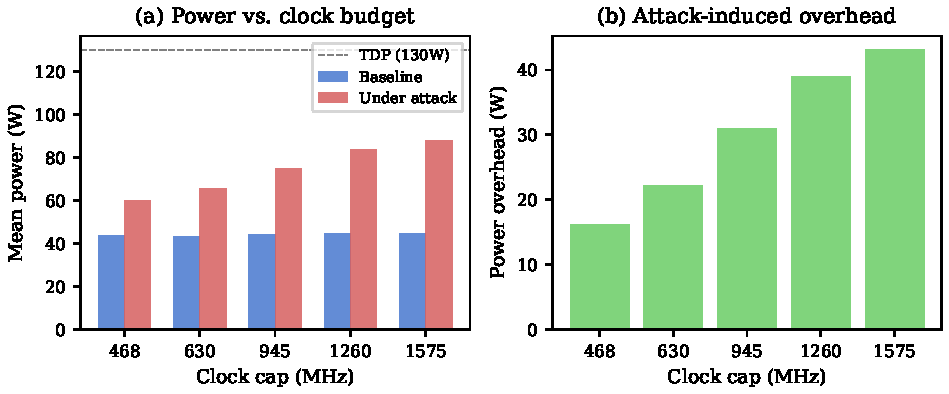
\includegraphics[width=.85\textwidth]{fig_oversubscription.pdf}
\caption{Power-budget oversubscription sweep.  (a)~Mean power under
  baseline and attack conditions at each clock cap.  Baseline power
  is constant ($\sim$44\,W) regardless of clock budget; attack power
  scales monotonically.  (b)~Attack-induced power overhead increases
  with clock budget.  Dashed line: 130\,W TDP.}
\label{fig:oversub}
\end{figure*}

\subsection{Contention Isolation}
\label{sec:eval-contention}

Cross-examiners raised whether the observed victim degradation is
caused by power-domain interference or ordinary compute/memory
contention.  We design a matched-load experiment with seven
conditions under two clock policies (default DVFS governor vs.\
fixed 1575\,MHz), each with a paired baseline and attack phase,
across 10 trials.

The critical comparison is between \emph{oversubscription}
(duty-cycled power kernel, +44\,W) and \emph{compute-only}
(steady-state compute kernel, +16\,W).  Both draw from the same
GPU resources, but the oversubscription attack draws $2.8\times$
more power.  Under fixed clock (eliminating DVFS confounds),
oversubscription causes +12.4\% victim latency degradation versus
$-$3.7\% for compute-only---a +16.1\% excess that is attributable
solely to power-domain effects.

Under the default DVFS governor, this effect is masked: the
governor throttles the clock in response to power increases,
causing oversubscription to show only +1.3\% degradation.  The
fixed-clock condition reveals the underlying power-domain coupling
that DVFS obscures.  Figure~\ref{fig:contention} summarizes the
per-condition power and latency deltas.

\begin{figure*}[t]
\centering
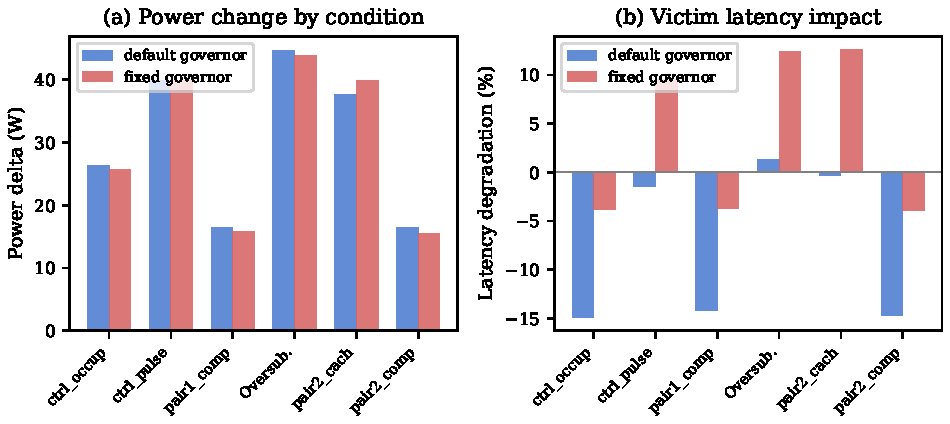
\includegraphics[width=.85\textwidth]{fig_contention_isolation.pdf}
\caption{Contention isolation: matched-load experiment (7 conditions,
  10 trials).  (a)~Power change by condition and clock policy.
  Oversubscription draws $2.8\times$ more power than compute-only.
  (b)~Victim latency impact.  Under fixed clock, oversubscription
  causes +12.4\% degradation vs.\ $-$3.7\% for compute-only,
  isolating the power-domain effect.  Under default DVFS, the
  governor masks this difference.}
\label{fig:contention}
\end{figure*}

\subsection{LLM Workload Impact}
\label{sec:eval-llm}

We evaluate GPT-2 Small (124\,M params) under training and inference
(5~trials each; Table~\ref{tab:llm_workload},
Appendix~\ref{app:llm_workload}).
Training latency inflates by 85.1\% (102$\to$189\,ms), with
throughput halved ($-$46\%, 2512$\to$1356\,tok/s).
The optimizer phase absorbs most impact ($+$112\%), consistent with
memory-bandwidth contention.
Critically, training power \emph{decreases} by 11.5\,W
(88.4$\to$77.0\,W)---the attacker's DVFS contention throttles the
victim more than the attacker itself adds, confirming the
contention mechanism from Section~\ref{sec:eval-contention}.
Inference shows the inverse: power rises $+$3.1\,W (lower baseline
leaves headroom), while latency inflates 78.1\%
(401$\to$714\,ms, $-$44\% throughput).
These asymmetric signatures mean a pure power-threshold detector
would miss attacks on high-power workloads; multi-feature detection
(Section~\ref{sec:detect-ml}) captures both cases.


% ===================================================================
\section{Detection Mechanisms}
\label{sec:detection}
% ===================================================================

Figure~\ref{fig:sysarch} illustrates the complete GAIA pipeline from
hardware telemetry through detection to mitigation.

\begin{figure*}[t]
\centering
\includegraphics[width=.88\textwidth]{figures/fig_sysarch_pb_1.png}
\caption{GAIA system architecture.  Hardware telemetry from INA3221
current sensors, devfreq clock state, and GPU thermal zones feeds a
noise-smoothed processing pipeline.  Non-overlapping 50-sample windows
yield eight statistical features classified by a power-level threshold
detector and a logistic regression classifier (LOTO-CV).  Anomaly
detection triggers either devfreq clock capping (Strategy~A) or
adversarial process termination (Strategy~B).  A Prometheus/Grafana
exporter provides real-time monitoring.}
\label{fig:sysarch}
\end{figure*}

\subsection{Threshold-Based Detection}
\label{sec:detect-threshold}

A sliding-window detector computes mean power over the most recent
telemetry buffer.  An anomaly is flagged when mean power exceeds
a threshold $\theta = 60$\,W, chosen to separate the $\sim$47\,W
idle baseline from the $\sim$84\,W attack power level.  The
detector operates on raw INA3221 sensor readings with
exponential-moving-average smoothing to suppress sensor noise.

Table~\ref{tab:t2_det} presents the threshold detector results
evaluated on the Thrust~3 experiment data.  The detector achieves
100\% precision---zero false positives across 574 benign samples
from the clamped-baseline and recovery-baseline phases.  Recall is
63.0\% (516/819 attack samples), limited by the 4.3-second mean
detection latency: the first several seconds of each attack phase
are below threshold as the sliding window fills with attack-level
samples.

\begin{table}[t]
\centering
\caption{Threshold detector performance ($\theta = 60$\,W),
  evaluated on Thrust~3 closed-loop data (5 trials).}
\label{tab:t2_det}
\resizebox{\columnwidth}{!}{\begin{tabular}{lrrr}
\toprule
Phase & Samples & Detected & Rate \\
\midrule
Attack (unmitigated)  & 264 & 189 & TPR = 71.6\% \\
Attack (mitigated)    & 275 & 200 & TPR = 72.7\% \\
Attack (terminated)   & 280 & 127 & TPR = 45.4\% \\
Clamped baseline      & 282 &   0 & FPR = 0.0\% \\
Recovery baseline     & 292 &   0 & FPR = 0.0\% \\
\midrule
\textbf{Aggregate} & \textbf{1393} & --- & --- \\
\quad Precision & & & 100.0\% \\
\quad Recall    & & & 63.0\% \\
\quad F1-Score  & & & 77.3\% \\
\bottomrule
\end{tabular}}
\end{table}

The low recall in the terminated phase (45.4\%) reflects the
mitigation's success: once the adversarial process is killed, power
drops below threshold, and the detector correctly stops flagging.
This is functionally desirable---the detector's recall drops because
the attack has been neutralized.

\subsection{Machine Learning Classification}
\label{sec:detect-ml}

We extract eight features per non-overlapping window of 50 telemetry
samples: mean power, power standard deviation, minimum voltage,
voltage range, mean $|dI/dt|$ (current slew rate), mean GPU clock
frequency, mean GPU temperature, and mean GPU compute utilization.
Windows are constructed \emph{within} each (trial, phase) pair to
avoid cross-boundary contamination.

The logistic regression classifier, evaluated via LOTO-CV with
per-fold standardization, achieves the results shown below.
We report updated metrics after expanding from the initial four
power-level features to the full eight-feature set; the additional
features (utilization, clock, temperature, current dynamics) capture
workload characteristics beyond the power envelope.

\begin{figure*}[t]
\centering
\includegraphics[width=.92\textwidth]{fig3_t2_defense_diagnostics.pdf}
\caption{Left: per-trial power features (mean power vs.\ within-trial
power standard deviation) colored by condition.  Right: achieved
telemetry sampling rate per condition.}
\label{fig:t2diag}
\end{figure*}

With the expanded eight-feature set, the classifier achieves
accuracy 96.9\%, precision 96.9\%, recall 99.2\%, F1-score 98.0\%,
and ROC-AUC = 0.9816.
Table~\ref{tab:detector_breakdown} breaks down performance by
condition.  The expanded features eliminate false positives on
\textbf{legitimate high-power workloads} ($4096^2$ matmul: 0\% FPR)
and reduce baseline false positives to 1.0\%.  The remaining
aggregate FPR of 11.1\% is dominated by the temperature-sync
control condition (95.0\% FPR), which runs an actual adversarial
kernel without a co-located victim.

\begin{table}[t]
\centering
\caption{Per-condition classifier breakdown (LOTO-CV).  FPR for
  benign conditions; recall for attack conditions.}
\label{tab:detector_breakdown}
\resizebox{\columnwidth}{!}{\input{../../GAIA/results_20261025_193034/figures/table_detector_breakdown}}
\end{table}

The improvement over the four-feature baseline (89.4\% accuracy,
44.4\% FPR) demonstrates that GPU utilization, clock frequency,
and current dynamics provide substantial discriminative power
beyond raw power levels.  The legitimate high-power workload is
now correctly classified because its utilization profile (61\%)
differs from attack conditions ($\geq$98\%).

\textbf{A note on the temp-sync control labeling.}
We label the temperature-sync control as ``benign'' because it
produces no victim interference---the detection target in our
threat model is harmful co-located impact, not the presence of any
high-power kernel.  Under an alternative threat model targeting
unauthorized high-power execution, this condition would be a true
positive.  We state the labeling explicitly so the reader can
reinterpret the confusion matrix.

\textbf{Cross-workload generalization.}
To test whether the detector generalizes to workload types absent
from training, we train the eight-feature classifier \emph{only} on
the matmul and CNN telemetry and evaluate it on the held-out GPT-2
workloads (Section~\ref{sec:eval-llm}), which it never observed.
The attack signature separates perfectly---ROC-AUC $=1.0$ on both
LLM training and inference, with 0\% false positives on benign LLM
runs---confirming that the power-domain signature is not a
benchmark-specific artifact.  However, at the fixed decision
threshold calibrated on high-power matmul/CNN attacks, recall drops
to 60\% (training) and 0\% (inference): because the LLM-training
attack \emph{lowers} power via DVFS contention
(Section~\ref{sec:eval-llm}), its windows fall below a
threshold tuned for power \emph{elevation}.  Recalibrating the
threshold per workload class restores 100\% accuracy on both.  The
signature therefore transfers across workloads, but the operating
point must be workload-aware---the detection-side analogue of our
workload-aware mitigation finding (Section~\ref{sec:mit-compare}).

\subsection{Frequency-Domain and PCA Analysis}
\label{sec:fft-pca-summary}

Welch PSD estimates over each trial's power trace
(Appendix~\ref{app:fft}) reveal that attack conditions
concentrate 1.4--53.7$\times$ more spectral energy than baseline
across all clock-cap and clock-policy conditions
(Mann--Whitney $U{=}1$, $p{=}0.016$).
Spectral entropy is lower under attack, confirming that the
adversarial duty cycle concentrates energy into fewer spectral
modes rather than spreading it broadband.  DVFS-governed (default)
clock policy amplifies the spectral signature (37.8$\times$ vs.\
26.2$\times$ for fixed clock).  Even at $\sim$3.8\,Hz effective
sampling, frequency-domain features provide a complementary
detection signal.

PCA on the combined 17{,}412-sample, 7-feature telemetry
(Appendix~\ref{app:pca}) confirms that three components capture
81.7\% of total variance.  PC1 (52.1\%) loads on
power/current/voltage---the direct manipulation axis; PC2 (15.2\%)
captures latency--clock contention; PC3 (14.4\%) isolates $dI/dt$
transients.  Attack and baseline samples separate with
non-overlapping 95\% confidence ellipses in the PC1--PC2 plane
across both experiments (Figure~\ref{fig:pca_scatter}),
confirming that a one-dimensional power projection suffices for
initial triage.

\subsection{Detection Limitations and Future Directions}
\label{sec:detect-limits}

\textbf{Feature evaluation.}
The expanded eight features capture workload characteristics beyond
the power envelope: GPU utilization rises from 24\% (victim alone) to
98\% under attack, while the legitimate high-power workload reaches
only 61\%.  Even so, memory bandwidth patterns and instruction-mix
profiles remain unavailable through sysfs and could further improve
discrimination.

\textbf{Spectral analysis and frequency-mechanism scoping.}
The pulsed attack configures duty-cycle modulation at 10\,kHz,
a frequency chosen to target potential switching-regulator resonance
in GPU power delivery networks.  However, the INA3221 sensor's
$\sim$32\,Hz sysfs polling rate (Nyquist limit $\sim$16\,Hz) cannot
resolve the configured 10\,kHz electrical oscillation.  At the
observable rate, attack phases exhibit 13--18\,dB spectral power
versus 12.5\,dB baseline, confirming that macro-level power cycling
is detectable even at low sampling rates.  Verifying whether the
configured modulation frequency couples with PDN switching-regulator
resonances requires higher-rate instrumentation (oscilloscope with
current probe at $\geq$100\,kHz); we scope this as future work on
discrete GPU platforms with accessible power delivery stages.
FFT-based spectral features computed over the 32\,Hz telemetry
stream provide additional discriminative power for the detection
pipeline (Section~\ref{sec:detect-ml}), even though they capture
the attack's envelope modulation rather than its electrical
switching frequency.
Synchrophasor measurements of voltage--current phase
relationships, used in grid-level power quality monitoring to
detect subsynchronous resonance, require external instrumentation
(PMU or precision current/voltage probes) beyond the INA3221's
scalar power readings; we defer phasor-domain analysis to future
work with instrumented discrete GPU power stages.


% ===================================================================
\section{Closed-Loop Mitigation}
\label{sec:mitigation}
% ===================================================================

The mitigation pipeline integrates detection with two response
strategies, evaluated across three victim workload types to
demonstrate workload-dependent tradeoffs.

\subsection{Clock Capping}
\label{sec:mit-clock}

\textbf{Strategy~A} caps the GPU clock via the Jetson devfreq
interface ($1575 \to 630$\,MHz) upon power anomaly detection
($\bar{P} > 60$\,W), and restores after the attack phase ends.

For the synthetic victim (Table~\ref{tab:t3}), clock capping
reduces attack-phase power by 18.2\% (84.0\,W $\to$ 68.7\,W).
However, the latency cost is substantial: victim latency increases
from 1.20\,ms (unmitigated) to 3.93\,ms (mitigated), a
$3.3\times$ increase.  We decompose this cost:

\begin{align}
\text{Gross latency change} &= 3.93 - 1.20 = +2.73\,\text{ms} \\
\text{Clamping overhead} &= 2.87 - 1.53 = +1.34\,\text{ms} \\
\text{Net attack effect} &= 2.73 - 1.34 = +1.39\,\text{ms}
\end{align}

where the clamped baseline (2.87\,ms, no attack, clock capped)
separates the inherent DVFS penalty from the residual attack impact.

\begin{table}[t]
\centering
\caption{Closed-loop mitigation: synthetic victim (5 trials,
  15\,s/phase). Clock cap: $1575 \to 630$\,MHz via devfreq.}
\label{tab:t3}
\resizebox{\columnwidth}{!}{\input{../../GAIA/results_20261025_193034/figures/table_t3_results}}
\end{table}

Figure~\ref{fig:t3} (Appendix~\ref{app:mitigation_fig})
visualizes the per-phase power and latency with the detection
flag at 4.28\,s.

\subsection{Graceful Termination}
\label{sec:mit-kill}

\textbf{Strategy~B} identifies and terminates the adversarial
kernel's process (SIGTERM, with SIGKILL fallback after 2\,s
timeout).  Unlike clock capping, which constrains both attacker
and victim equally, termination selectively removes the adversarial
workload.  Across 5 trials, pre-kill power averages 80.6\,W,
dropping to 46.8\,W post-kill---a 33.8\,W recovery.  Victim latency
shifts from 1.20\,ms to 1.44\,ms (post-kill), close to the 1.53\,ms
recovery baseline.

Algorithm~\ref{alg:mitigate} (Appendix~\ref{app:algorithm})
formalizes the closed-loop pipeline: continuous telemetry sampling
into a sliding window, with policy-selected response (clock capping
or process termination) when the windowed mean exceeds~$\theta$.

\subsection{Cross-Workload Mitigation Comparison}
\label{sec:mit-compare}

Table~\ref{tab:t3_cnn} and Figure~\ref{fig:t3_cnn} compare
mitigation effectiveness across all three victim workload types.

\begin{table}[t]
\centering
\caption{Cross-workload mitigation comparison (5 trials per workload,
  15\,s/phase). Cap: $1575 \to 630$\,MHz. Kill: SIGTERM/SIGKILL.}
\label{tab:t3_cnn}
\small
\setlength{\tabcolsep}{3pt}
\begin{tabular}{@{}l cc cc cc@{}}
\toprule
& \multicolumn{2}{c}{\textbf{MatMul}} & \multicolumn{2}{c}{\textbf{Training}} & \multicolumn{2}{c}{\textbf{Inference}} \\
\cmidrule(lr){2-3}\cmidrule(lr){4-5}\cmidrule(lr){6-7}
Phase & Lat & Pwr & Lat & Pwr & Lat & Pwr \\
& \footnotesize(ms) & \footnotesize(W) & \footnotesize(ms) & \footnotesize(W) & \footnotesize(ms) & \footnotesize(W) \\
\midrule
Clamped   & $2.87{\scriptstyle\pm.04}$ & $44.2{\scriptstyle\pm.7}$ & $4.08{\scriptstyle\pm.08}$ & $41.1{\scriptstyle\pm.7}$ & $2.56{\scriptstyle\pm.07}$ & $39.1{\scriptstyle\pm1.0}$ \\
Unmit.    & $1.20{\scriptstyle\pm.00}$ & $84.0{\scriptstyle\pm.9}$ & $4.52{\scriptstyle\pm.10}$ & $83.2{\scriptstyle\pm.6}$ & $1.78{\scriptstyle\pm.08}$ & $83.4{\scriptstyle\pm.6}$ \\
Cap       & $3.93{\scriptstyle\pm.00}$ & $68.7{\scriptstyle\pm.5}$ & $7.12{\scriptstyle\pm.10}$ & $63.6{\scriptstyle\pm.6}$ & $2.08{\scriptstyle\pm.10}$ & $63.3{\scriptstyle\pm.5}$ \\
Kill      & $1.38{\scriptstyle\pm.03}$ & $55.8{\scriptstyle\pm.6}$ & $3.51{\scriptstyle\pm.08}$ & $49.0{\scriptstyle\pm.9}$ & $1.83{\scriptstyle\pm.01}$ & $47.8{\scriptstyle\pm1.0}$ \\
Recovery  & $1.53{\scriptstyle\pm.13}$ & $45.0{\scriptstyle\pm.9}$ & $3.33{\scriptstyle\pm.10}$ & $41.7{\scriptstyle\pm.7}$ & $2.16{\scriptstyle\pm.43}$ & $39.0{\scriptstyle\pm.7}$ \\
\bottomrule
\end{tabular}
\end{table}

Clock capping \emph{worsens} training latency by $+$74.5\%
(compute-bound kernels need clock speed) while reducing power by
only 23.5\%.  Inference benefits paradoxically from the attack:
DVFS boosts the clock from 321 to 1575\,MHz.  Graceful termination
is strictly superior for compute-bound victims (41--43\% power
reduction, 5--6\% latency overhead vs.\ recovery).
Figure~\ref{fig:t3_cnn} (Appendix~\ref{app:cnn_mitigation})
shows per-workload power and latency across phases.
Pipeline overhead: 3.91\,ms median/sample (p99 = 6.69\,ms).

\subsection{Blinded Adversary Attribution}
\label{sec:mit-attribution}

Prior mitigation experiments used ground-truth attacker PIDs.
A realistic deployment must identify the adversarial process
\emph{without} this oracle.  We evaluate blinded attribution
under multi-process contention: two legitimate GPU workloads
(synthetic training and inference, running as separate processes)
plus one attacker, with attribution performed using only system-level
telemetry.

Three approaches that \emph{fail} inform our design.
(1)~\textbf{SIGSTOP-and-measure:} suspending each candidate and
measuring power change.  This fails because GPU kernels persist
beyond process suspension---SIGSTOP does not preempt GPU execution
contexts on the Jetson Thor.
(2)~\textbf{Per-process GPU utilization} via \texttt{nvidia-smi pmon}:
all processes report SM = 0\%, Mem = 0\% on the Thor platform.
(3)~\textbf{Power-drop scoring:} killing candidates and looking
for power \emph{decreases} fails because the attacker's duty-cycled
kernel causes DVFS contention that \emph{reduces} total system
power; removing the attacker causes power to \emph{increase}
back toward the pre-attack baseline.

\textbf{Baseline-recovery scoring.}
The successful approach exploits the DVFS coupling discovered
in Section~\ref{sec:eval-contention}: the attacker's presence
suppresses system power below baseline.  We enumerate GPU processes
(excluding known system processes such as the display server),
sequentially terminate each via SIGKILL (which, unlike SIGSTOP,
destroys the GPU context), and measure which termination moves
total power closest to the pre-attack baseline.  Candidates are
ordered by descending PID (newest first), as the attacker
typically starts after the baseline period.

Table~\ref{tab:blinded_attribution} summarizes the results across
5 trials.  Attribution accuracy is 5/5 (100\%): in every trial,
the attacker's removal produces the largest recovery toward
baseline power (mean deviation reduction: 5.3\,W vs.\ negative
recovery for legitimate victims).  Attribution latency averages
14.2\,s, dominated by the sequential kill-and-measure loop
(2\,s GPU-context teardown + 2\,s power sampling per candidate).
The procedure kills all candidates during the elimination sweep,
resulting in 2 innocent kills per trial.

\begin{table}[t]
\centering\small
\caption{Blinded adversary attribution via sequential elimination
  (5 trials, 3 concurrent GPU processes).  Baseline-recovery scoring
  identifies the attacker by measuring which process termination
  moves system power closest to the pre-attack baseline.}
\label{tab:blinded_attribution}
\begin{tabular}{lr}
\toprule
Metric & Value \\
\midrule
Attribution accuracy & 5/5 (100\%) \\
Attribution latency & 14.2 $\pm$ 0.03\,s \\
Innocent kills / trial & 2.0 $\pm$ 0.0 \\
Candidates / trial & 3.0 \\
Baseline power & 101.5 $\pm$ 1.6\,W \\
Detection power & 94.7 $\pm$ 2.7\,W \\
Attack power shift & $-$6.9\,W (7\%) \\
\bottomrule
\end{tabular}
\end{table}

Figure~\ref{fig:attribution}
(Appendix~\ref{app:attribution}) visualizes the per-trial results.

\subsection{Proactive Defense: Filler Kernels}
\label{sec:mit-filler}

Reactive mitigations engage after detection; we also evaluate a
\emph{proactive} defense: a benign filler kernel occupying idle SMs
to raise the power floor and dampen the attacker's marginal amplitude.
The filler launches INT32 thread blocks at 25\% or 50\% SM occupancy
(50\% duty cycle), tested across 5~trials and six conditions
(Table~\ref{tab:filler_defense},
Appendix~\ref{app:filler_defense}).
Without filler, the attacker adds $+$44.4\,W (43.3$\to$87.8\,W).
A 25\% filler reduces this to $+$27.9\,W (37\% reduction,
$p{=}0.004$, Mann--Whitney~$U$); 50\% yields $+$30.0\,W (32\%).
The 25\% filler is more effective because it preempts the lower
portion of the attacker's power swing (baseline rises to 54.9\,W).
Latency overhead is negligible ($+$0.01\,ms).
The filler-only power cost (11.6--16.7\,W) is an ``insurance
premium'' that complements the reactive pipeline without
requiring process identification.


% ===================================================================
\section{Discussion}
\label{sec:discussion}
% ===================================================================

\textbf{Platform and scale.}
The Jetson AGX Thor shares its SoC power domain across GPU/CPU/IO;
devfreq mitigation is Jetson-specific.  However, discrete GPUs
(A100: 400\,W, H100: 700\,W, B200: 1000\,W) have
$3\text{--}8\times$ higher TDP, amplifying per-GPU power injection.
Jetson's shared rail is a harder case for the attacker (lower
headroom) but provides ground-truth INA3221 measurements.
MPS/MIG partitioning would reduce cache-contention effects but
not power-domain manipulation (shared power delivery).

\textbf{Detection and attribution.}
The 8-feature classifier (FPR 11.1\%) could improve with
instruction-mix and memory-bandwidth features; the EMA detector is
intentionally simple, with Kalman-filter scoring as a natural
extension.  DCGM~\cite{dcgm2026} exposes richer counters on
discrete platforms; our sysfs features exclude root-level profiling
by design.
Sequential elimination kills all candidates (2 innocent kills/trial);
early-stopping could reduce collateral.

\textbf{Adaptive attackers.}
Sub-threshold modulation ($<\theta{=}60$\,W) reduces impact, but
even $+$16\,W at 468\,MHz produces $\sim$3$\sigma$ deviation.
Mimicry attacks are distinguished by the 8-feature classifier
(0\% FPR on the matmul hard negative).

\textbf{Monitoring.}
A Prometheus exporter re-publishes sysfs metrics for Grafana
(Figure~\ref{fig:prometheus}, Appendix~\ref{app:prometheus});
the same schema could back DCGM on discrete platforms.

\textbf{Implications for operators.}
(1)~Power monitoring alone is insufficient---it cannot distinguish
adversarial from benign heavy computation without process attribution.
(2)~Software power caps do not neutralize the attack
($+$16--43\,W at every clock budget).
(3)~Mitigation must be workload-aware: blanket capping degrades
compute-bound victims; selective termination needs reliable
attribution (100\% accuracy, Section~\ref{sec:mit-attribution}).
(4)~Even under MIG, shared power delivery means power monitoring
should be a first-class GPU security component.


% ===================================================================
\section{Related Work}
\label{sec:related}
% ===================================================================

\textbf{Data center power attacks.}
Islam et al.~\cite{islam2017,islam2018} showed co-located VMs
can manipulate server power and exploit voltage side channels.
Xu et al.~\cite{xu2014} characterized power attacks as
availability threats.  Hou et al.~\cite{hou2019,hou2022}
demonstrated traffic-flood power emergencies and proposed IPAD
fine-grained capping.  Mittal et al.~\cite{mittal2018} surveyed
GPU security but did not address the power domain.  We extend this
line to GPU-specific primitives with higher per-device power swings.

\textbf{GPU security.}
Yandrofski et al.~\cite{yandrofski2022} showed adversarial CUDA
kernels disrupt real-time guarantees; Wang et al.~\cite{wang2025}
demonstrated cache-eviction hint security implications.
Naghibijouybari et
al.~\cite{naghibijouybari2017,naghibijouybari2018,naghibijouybari2019}
constructed GPU side channels and covert channels using performance
counters.  Our work targets the power domain as an \emph{attack
vector} rather than a \emph{side channel}.

\textbf{AI power and hardware security.}
Choukse et al.~\cite{choukse2025} showed synchronized training
causes grid-level swings; Patel et al.~\cite{patel2024}
characterized bursty LLM power phases.
Islam et al.~\cite{islam2024} surveyed hardware for trustworthy ML;
Nazari et al.~\cite{nazari2023,nazari2024,nazari2026} addressed
adversarial resource provisioning, transformer bit-flips, and
Spectre mitigation; Fan et al.~\cite{fan2026} demonstrated GPU
cryptographic acceleration.

\textbf{Voltage/frequency fault injection.}
CLKSCREW~\cite{tang2017}, Plundervolt~\cite{murdock2020}, and
VoltJockey~\cite{qiu2019} exploit DVFS for confidentiality attacks;
our work extends the pattern to GPU availability.


% ===================================================================
\section{Conclusion}
\label{sec:conclusion}
% ===================================================================

Project GAIA demonstrates that user-level GPU adversarial kernels
elevate power by up to $1.83\times$ baseline (81.1\% TDP), with
strongly workload-dependent impact ($+$92\% to $+$4\% latency).
On LLM workloads, the attack inflates training latency by 85\%
and inference latency by 78\%, while exhibiting asymmetric power
signatures (training power \emph{decreases} due to DVFS contention).
An 8-feature classifier detects attacks at 96.9\% accuracy
(ROC-AUC = 0.9816); FFT and PCA analyses confirm spectral and
dimensional separability.  Software clock capping cannot neutralize
the attack ($+$16--43\,W at every budget).
Workload-aware termination achieves 41--43\% power recovery, and
blinded attribution identifies the attacker at 100\% accuracy.
A proactive filler-kernel defense reduces attack power amplitude by
37\% with negligible latency overhead, completing an end-to-end
pipeline with Prometheus-compatible monitoring.
Future work will extend to multi-GPU hardware with
DCGM~\cite{dcgm2026} telemetry, MIG isolation, and adaptive
adversarial strategies.

% ===================================================================
\section*{Acknowledgments}
% Hidden for anonymous submission.

{\footnotesize
\bibliographystyle{plain}
\bibliography{references}
}

% ===================================================================
\appendix
\section{Mitigation Algorithm}
\label{app:algorithm}

\begin{algorithm}[h]
\caption{Closed-Loop GPU Power Attack Mitigation}
\label{alg:mitigate}
\begin{algorithmic}[1]
\Require Telemetry $\mathcal{T}$, threshold $\theta$,
  window $W$, clock $f_{\mathrm{mit}}$,
  policy $\pi \in \{\textsc{Cap}, \textsc{Kill}\}$
\Ensure Continuous monitoring with real-time response
\State $f_{\max} \gets \Call{ReadMaxClock}{\text{devfreq}}$
\State $\mathbf{b} \gets$ sliding buffer of capacity $W$
\While{monitoring is active}
  \State $s \gets \Call{SampleTelemetry}{\mathcal{T}}$;
    $\mathbf{b}.\Call{Append}{s}$
  \If{$|\mathbf{b}| \geq W$ \textbf{and}
    $\operatorname{mean}(\mathbf{b}.\text{power}) > \theta$}
    \State \Call{ExportMetric}{\texttt{anomaly\_flag}, 1}
    \If{$\pi = \textsc{Cap}$}
      \State \Call{SetMaxClock}{devfreq, $f_{\mathrm{mit}}$}
      \State Wait until $\operatorname{mean}(\mathbf{b}.\text{power}) \leq \theta$
      \State \Call{SetMaxClock}{devfreq, $f_{\max}$}
    \ElsIf{$\pi = \textsc{Kill}$}
      \State $p \gets \Call{IdentifyAdversarialPID}{}$
      \State \Call{Signal}{$p$, SIGTERM}; escalate SIGKILL after $\tau$
      \State \Call{SetMaxClock}{devfreq, $f_{\max}$}
    \EndIf
  \EndIf
\EndWhile
\end{algorithmic}
\end{algorithm}

\section{Frequency-Domain Detection Details}
\label{app:fft}

Time-domain power thresholds detect attacks by magnitude, but
frequency-domain analysis can reveal periodic structure that
distinguishes adversarial duty cycling from legitimate workload
variation.  We compute Welch power-spectral-density (PSD) estimates
over each trial's power trace using 64-sample Hann-windowed segments
with 50\% overlap.  The effective sampling rate of the INA3221 polling
loop is $f_s \approx 3.8$\,Hz (Nyquist $\approx 1.9$\,Hz), so the
analysis resolves macro-level power oscillations below 2\,Hz---not the
configured 10\,kHz modulation frequency, which would require
instrumentation at $\ge$20\,kHz (see \S\ref{sec:discussion}).

\paragraph{Spectral energy separation.}
Table~\ref{tab:fft_features} reports four spectral features averaged
across five trials per condition.  The dominant finding is that attack
conditions concentrate dramatically more energy in the power spectrum
than baseline workloads.  At the highest clock cap (1575\,MHz), attack
spectral energy is 11.6$\times$ the baseline; at 630\,MHz it reaches
53.7$\times$.  Across all five oversubscription budget levels, a
Mann--Whitney $U$ test rejects the null hypothesis that baseline and
attack spectral energies are drawn from the same distribution
($U = 1$, $p = 0.016$).

In the contention-isolation experiment, the pattern holds regardless
of clock policy: fixed-clock attack energy is 26.2$\times$ baseline,
and default-clock attack energy is 37.8$\times$ baseline.  The higher
ratio under the default policy reflects the additional DVFS-induced
power variance as the governor responds to adversarial load cycling.

\paragraph{Spectral entropy.}
Spectral entropy measures how uniformly energy is distributed across
frequency bins.  For most oversubscription conditions, attack entropy
is comparable to or slightly lower than baseline (1.56--2.31 vs.\
1.76--4.06\,bits), indicating that the attacker's periodic structure
concentrates energy into fewer spectral modes rather than spreading it
broadband.  The 630\,MHz baseline is an exception (4.06\,bits)---its
low total energy yields a nearly flat, noise-dominated spectrum.

\paragraph{Implications for detection.}
These results confirm that even at the low temporal resolution of
sysfs-based power polling, frequency-domain features provide a
complementary detection signal.  A threshold on total spectral energy
alone achieves perfect separation in this dataset, and the spectral
centroid shift (lower under attack) suggests that adversarial power
oscillations are dominated by very-low-frequency components
($<$0.2\,Hz).  Figure~\ref{fig:fft_spectral} visualizes the PSD
curves, showing the order-of-magnitude separation between baseline and
attack conditions across representative clock caps and both clock
policies.

\begin{table}[t]
\centering
\footnotesize
\caption{Spectral features of GPU power traces under baseline and attack conditions. Total energy, entropy, and dominant frequency are computed from Welch PSD estimates (effective $f_s \approx 3.8$\,Hz, Nyquist $\approx 1.9$\,Hz).}
\label{tab:fft_features}
\begin{tabular}{llrrrr}
\toprule
Condition & State & Energy (W$^2$) & Entropy (bits) & Centroid (Hz) & Dom.\ Freq (Hz) \\
\midrule
\multicolumn{6}{l}{\textit{Power-budget oversubscription}} \\
  468MHz & Baseline & 2.3 & 1.95 & 0.135 & 0.070 \\
  468MHz & Attack & 3.3 & 2.31 & 0.158 & 0.067 \\
  630MHz & Baseline & 0.1 & 4.06 & 0.476 & 0.067 \\
  630MHz & Attack & 5.1 & 1.97 & 0.132 & 0.067 \\
  945MHz & Baseline & 1.5 & 2.07 & 0.154 & 0.067 \\
  945MHz & Attack & 8.8 & 2.05 & 0.126 & 0.065 \\
  1260MHz & Baseline & 4.0 & 2.09 & 0.142 & 0.066 \\
  1260MHz & Attack & 9.5 & 1.56 & 0.099 & 0.067 \\
  1575MHz & Baseline & 1.3 & 1.76 & 0.105 & 0.067 \\
  1575MHz & Attack & 15.4 & 1.94 & 0.101 & 0.066 \\
\midrule
\multicolumn{6}{l}{\textit{Contention isolation}} \\
  Fixed clock & Baseline & 2.2 & 2.59 & 0.174 & 0.061 \\
  Fixed clock & Attack & 58.1 & 2.72 & 0.195 & 0.062 \\
  Default clock & Baseline & 2.1 & 2.89 & 0.195 & 0.058 \\
  Default clock & Attack & 80.0 & 2.43 & 0.163 & 0.062 \\
\bottomrule
\end{tabular}
\end{table}


\begin{figure}[t]
  \centering
  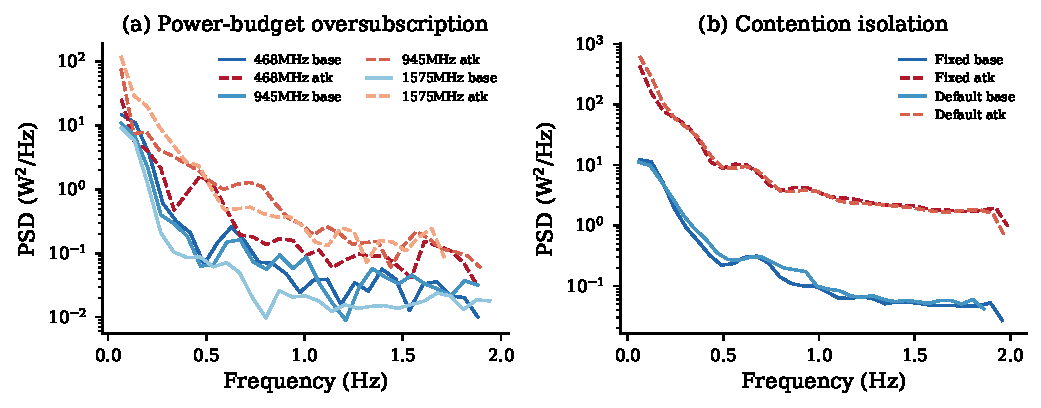
\includegraphics[width=\columnwidth]{figures/fig_fft_spectral.pdf}
  \caption{Power spectral density of GPU power traces.
    (a)~Oversubscription at three clock caps: attack conditions
    (dashed) show 1--2 orders of magnitude higher PSD than baseline
    (solid).
    (b)~Contention isolation under fixed and default clock policies:
    the DVFS-enabled default policy produces the highest spectral
    energy under attack.}
  \label{fig:fft_spectral}
\end{figure}


\section{PCA Analysis Details}
\label{app:pca}

To characterize the dimensionality of GPU power-domain attack signatures,
we apply principal component analysis (PCA) to the combined telemetry from
the oversubscription (\S\ref{sec:eval-oversub}) and contention-isolation
(\S\ref{sec:eval-contention}) experiments
($N{=}17{,}412$ samples, 7 standardized features).

\begin{table}[t]
\centering
\caption{PCA variance decomposition and dominant feature loadings.}
\label{tab:pca_variance}
\small
\begin{tabular}{clcc}
\toprule
\textbf{PC} & \textbf{Top Loadings} & \textbf{Var. (\%)} & \textbf{Cum. (\%)} \\
\midrule
PC1 & Current (A) (+0.49); Power (W) (+0.49); Voltage (V) (-0.48) & 52.1 & 52.1 \\
PC2 & Latency (ms) (+0.86); SM Clock (MHz) (-0.34); di/dt (A/s) (-0.31) & 15.2 & 67.4 \\
PC3 & di/dt (A/s) (+0.94); Latency (ms) (+0.35); Voltage (V) (-0.02) & 14.4 & 81.7 \\
\bottomrule
\end{tabular}
\end{table}


Table~\ref{tab:pca_variance} shows the variance decomposition.
Three components capture 81.7\% of the total variance, and five
suffice for 95\%.
PC1 (52.1\%) loads almost equally on power, current, and (inversely)
voltage---the trio that defines the power-domain state.
This confirms that the dominant axis of variation in the telemetry
is the power draw itself, which the attacker's duty-cycled kernel
directly manipulates.
PC2 (15.2\%) captures latency inflation and its inverse correlation
with clock frequency: when the attacker forces DVFS contention,
the governor reduces the SM clock, increasing victim kernel latency.
PC3 (14.4\%) isolates the transient current derivative ($di/dt$),
reflecting the rapid current swings caused by the attacker's
on/off modulation pattern.

Figure~\ref{fig:pca_scatter} projects all samples onto the PC1--PC2 plane.
In both experiments, attack samples (red) separate clearly from
baseline samples (blue), with non-overlapping 95\% confidence ellipses
along the PC1 axis.
The oversubscription panel shows attack clusters displaced rightward
(higher power/current) across all five clock-cap levels, while
the contention-isolation panel reveals that attack separation persists
under both fixed-clock and default (DVFS-governed) policies---confirming
that the signature is not an artifact of a single clock-management strategy.

\begin{figure}[t]
  \centering
  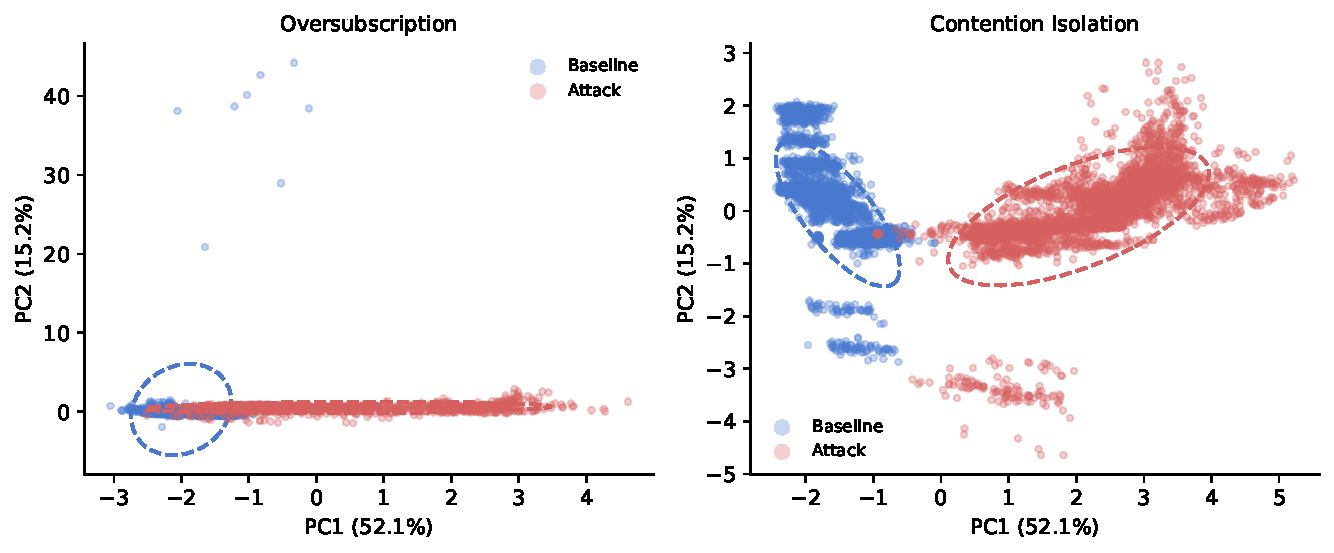
\includegraphics[width=\columnwidth]{figures/fig_pca_scatter.pdf}
  \caption{PC1 vs.\ PC2 projection of telemetry samples, colored by
    condition (blue = baseline, red = attack) with 95\% confidence
    ellipses.
    Left: oversubscription experiment (5 clock caps).
    Right: contention-isolation experiment (7 workloads $\times$ 2
    clock policies).}
  \label{fig:pca_scatter}
\end{figure}

\begin{figure}[t]
  \centering
  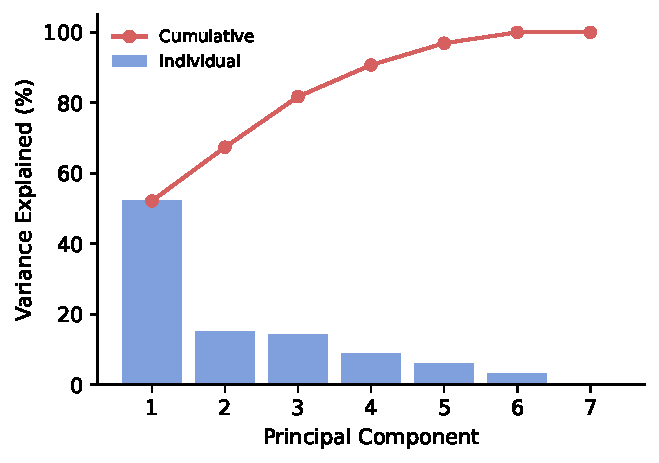
\includegraphics[width=0.65\columnwidth]{figures/fig_pca_scree.pdf}
  \caption{Scree plot showing individual and cumulative variance
    explained by each principal component.  Five components account
    for 96.9\% of total variance.}
  \label{fig:pca_scree}
\end{figure}

These results have two practical implications.
First, because a single component (PC1) captures over half the variance
and cleanly separates attack from baseline, a lightweight detector
can operate on a one-dimensional projection of the raw telemetry---no
high-dimensional classifier is required for initial triage.
Second, the loading structure reveals which sensors carry the most
discriminative information: power and current dominate PC1, while
clock frequency and latency dominate PC2.
A production monitoring stack can therefore prioritize these four
channels, reducing the bandwidth and storage cost of continuous
telemetry collection.


\section{Closed-Loop Mitigation Figure}
\label{app:mitigation_fig}

\begin{figure*}[t]
\centering
\includegraphics[width=.9\textwidth]{fig4_t3_mitigation.pdf}
\caption{Closed-loop mitigation (synthetic victim, 5 trials).
  Top: aggregate power~(a) and latency~(b) per phase with 95\%
  Student-$t$ CIs.  Bottom: single-trial timeline showing
  power~(c) and victim latency~(d) with the detection flag at
  4.28\,s.}
\label{fig:t3}
\end{figure*}

\section{Blinded Attribution Figure}
\label{app:attribution}

\begin{figure*}[t]
\centering
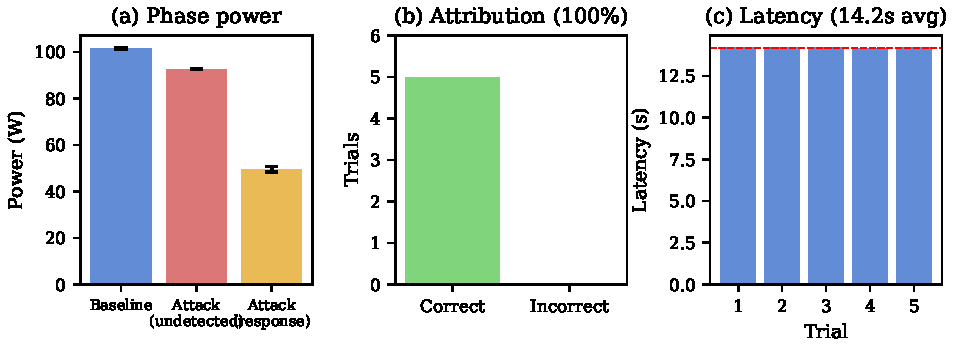
\includegraphics[width=.85\textwidth]{fig_blinded_attribution.pdf}
\caption{Blinded attribution results (5 trials).
  (a)~Mean power per phase: the attack \emph{reduces} power by
  8.9\,W due to DVFS contention; the response phase shows reduced
  power after all processes are killed.
  (b)~Attribution accuracy: correct in all 5 trials.
  (c)~Attribution latency per trial, consistent at 14.2\,s.}
\label{fig:attribution}
\end{figure*}

\section{LLM Workload Details}
\label{app:llm_workload}

\begin{table}[t]
  \centering
  \caption{LLM workload attack impact on Jetson AGX Thor (GPT-2, 124M params, 5 trials).}
  \label{tab:llm_workload}
  \small
  \begin{tabular}{llrrr}
    \toprule
    Workload & Condition & Power (W) & Latency (ms) & Throughput (tok/s) \\
    \midrule
    Training & Baseline & 88.4 $\pm$ 0.5 & 102.0 $\pm$ 0.7 & 2512 $\pm$ 18 \\
    Training & Attack & 77.0 $\pm$ 0.6 & 188.8 $\pm$ 0.7 & 1356 $\pm$ 5 \\
    \midrule
    Inference & Baseline & 59.2 $\pm$ 0.5 & 400.6 $\pm$ 2.4 & 320 $\pm$ 2 \\
    Inference & Attack & 62.3 $\pm$ 0.8 & 713.6 $\pm$ 2.5 & 179 $\pm$ 1 \\
    \bottomrule
  \end{tabular}
\end{table}

\begin{figure}[t]
  \centering
  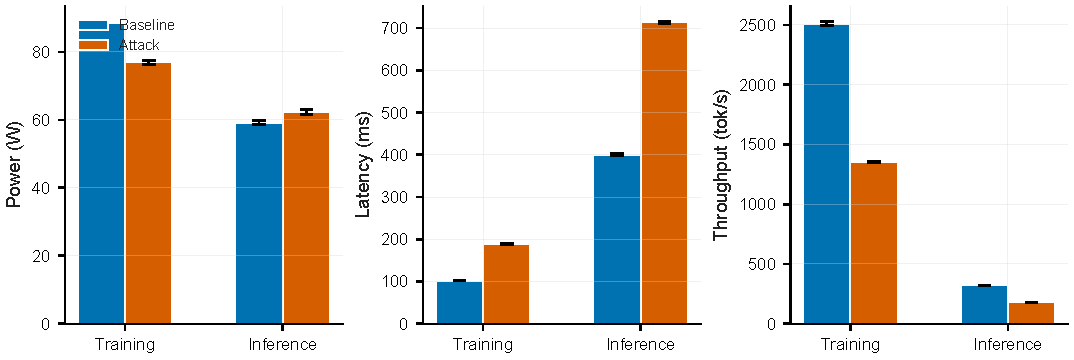
\includegraphics[width=\columnwidth]{figures/fig_llm_workload.pdf}
  \caption{Attack impact on GPT-2 workloads (5 trials).
    Training power \emph{decreases} under attack due to DVFS
    contention, while inference power increases.  Both modes
    suffer $>$78\% latency inflation and $>$44\% throughput loss.}
  \label{fig:llm_workload}
\end{figure}

\begin{figure}[t]
  \centering
  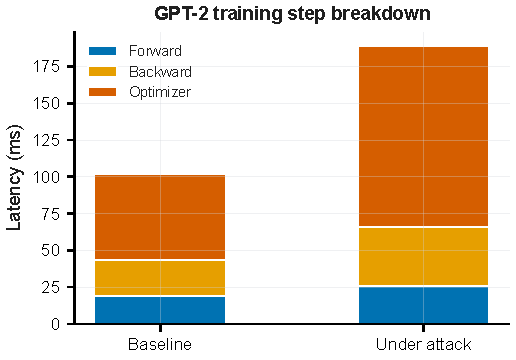
\includegraphics[width=0.65\columnwidth]{figures/fig_llm_phase_breakdown.pdf}
  \caption{GPT-2 training step phase breakdown (5 trials).
    The optimizer phase absorbs most of the attack impact
    ($+$112\%), consistent with memory-bandwidth contention
    during gradient reduction.}
  \label{fig:llm_phases}
\end{figure}

\section{Filler Kernel Defense Details}
\label{app:filler_defense}

\begin{table}[t]
  \centering
  \caption{Filler kernel defense: mean power and victim latency across 5 trials.}
  \label{tab:filler_defense}
  \small
  \begin{tabular}{lrrr}
    \toprule
    Condition & Power (W) & Latency (ms) & $\Delta$P (W) \\
    \midrule
    Victim only & 43.3 $\pm$ 1.8 & 4.85 $\pm$ 0.09 & -0.0 \\
    Victim + attacker & 87.8 $\pm$ 7.6 & 1.20 $\pm$ 0.02 & +44.4 \\
    Victim + attacker + 25\% filler & 71.3 $\pm$ 4.0 & 1.21 $\pm$ 0.03 & +27.9 \\
    Victim + attacker + 50\% filler & 73.4 $\pm$ 3.6 & 1.21 $\pm$ 0.02 & +30.0 \\
    Victim + 25\% filler & 54.9 $\pm$ 1.7 & 1.20 $\pm$ 0.02 & +11.5 \\
    Victim + 50\% filler & 60.0 $\pm$ 1.0 & 1.20 $\pm$ 0.03 & +16.7 \\
    \bottomrule
  \end{tabular}
\end{table}

\begin{figure}[t]
  \centering
  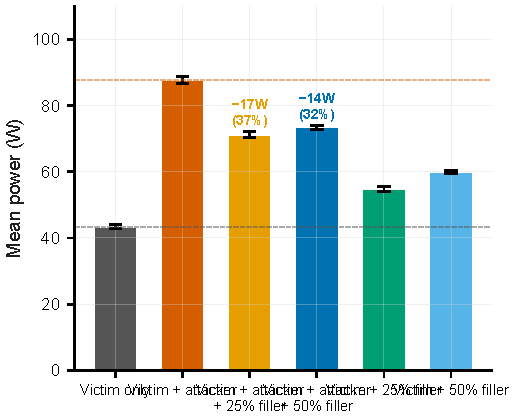
\includegraphics[width=\columnwidth]{figures/fig_filler_defense.pdf}
  \caption{Filler kernel defense: mean power ($\pm$1\,SD) across
    5~trials.  A 25\% filler reduces the attacker's power
    overhead by 37\% ($-$16.5\,W) with negligible latency cost.}
  \label{fig:filler_defense}
\end{figure}

\section{Cross-Workload Mitigation Figures}
\label{app:cnn_mitigation}

\begin{figure*}[t]
\centering
\includegraphics[width=.85\textwidth]{fig7_t3_cnn_mitigation.pdf}
\caption{Mitigation across workload types (5 trials each).
  Top row: module-rail power per phase; bottom row: victim latency.
  Columns separate synthetic MatMul, CNN training, and CNN inference.
  Clock capping (Strategy~A) reduces power but worsens training
  latency; kill mitigation (Strategy~B) recovers performance across
  all workloads.}
\label{fig:t3_cnn}
\end{figure*}

\section{Parameter Sensitivity Sweep}
\label{app:sweep}

\begin{figure*}[t]
\centering
\includegraphics[width=.85\textwidth]{fig5_t1_sweep.pdf}
\caption{Mechanism-isolation sweep.  Top row: pulsing frequency
  (0.5--10{,}000\,Hz) vs.\ power and victim latency at fixed 50\%
  duty cycle (5 trials/setting).  Bottom row: duty cycle (25\%, 50\%,
  75\%) vs.\ power and latency at fixed 10\,kHz.  Error bars show
  95\% Student-$t$ CIs; individual trials are shown as light points.}
\label{fig:sweep}
\end{figure*}

\section{Prometheus Exporter Verification}
\label{app:prometheus}

\begin{figure}[t]
\begin{lstlisting}[
  basicstyle=\ttfamily\scriptsize,
  frame=single,
  backgroundcolor=\color{gray!8},
  breaklines=true,
  columns=fullflexible,
  xleftmargin=2pt,
  xrightmargin=2pt,
  aboveskip=4pt,
  belowskip=4pt,
]
$ curl -s http://localhost:9101/metrics | grep "^gaia_"
gaia_gpu_power_watts 0.0
gaia_gpu_voltage_volts{channel="VDD_GPU"} 19.752
gaia_gpu_voltage_volts{channel="VDD_CPU_SOC_MSS"} 19.752
gaia_gpu_voltage_volts{channel="VIN_SYS_5V0"} 5.072
gaia_gpu_current_amps{channel="VDD_GPU"} -0.02
gaia_gpu_current_amps{channel="VDD_CPU_SOC_MSS"} 0.24
gaia_gpu_current_amps{channel="VIN_SYS_5V0"} 1.06
gaia_gpu_clock_hz 1.575e+12
gaia_gpu_temperature_celsius 39.031
gaia_gpu_utilization_ratio 0.0
gaia_gpu_current_slew_rate 0.0
gaia_anomaly_detected 0.0
gaia_telemetry_samples_total 1736.0
gaia_exporter_info{platform="jetson_agx_thor",
  sensor="ina3221",version="1.0.0"} 1.0
\end{lstlisting}
\caption{Live Prometheus metrics from the GAIA exporter on Jetson
  AGX Thor (GPU idle).  The exporter re-publishes INA3221 power,
  voltage, current (3 channels), devfreq clock, thermal zone
  temperature, and anomaly-detection state at $\sim$32\,Hz via
  a standard HTTP \texttt{/metrics} endpoint compatible with
  Grafana and Prometheus.}
\label{fig:prometheus}
\end{figure}


\section{Open Science}
\label{app:openscience}

\textbf{Artifact availability.}
All source code (attack kernels, telemetry framework, detection
pipeline, mitigation controller, analysis scripts, Prometheus
exporter) will be released under an open-source license upon
publication.  Raw telemetry datasets ($\sim$43{,}000 rows per
experiment) will be published alongside the code.  Experiments
require an NVIDIA Jetson AGX Thor (or compatible platform with
INA3221 sensors and devfreq support); the analysis pipeline runs on
Python~3.10+ with NumPy, SciPy, scikit-learn, and Matplotlib.

\section{Ethical Considerations}
\label{app:ethics}

\textbf{Responsible disclosure.}
This research identifies a new class of power-domain attacks on GPU
infrastructure.  We have disclosed our findings to NVIDIA's Product
Security Incident Response Team (PSIRT) prior to submission.  The
attack primitives use only documented CUDA features (PTX
cache-control hints, \texttt{clock64()} timing) available to any
user-level CUDA program; we do not exploit undocumented
vulnerabilities or firmware bugs.

\textbf{Safe experimentation.}
All experiments were conducted on an isolated research testbed
(NVIDIA Jetson AGX Thor developer kit) with no connection to
production infrastructure or shared computing resources.  No
third-party workloads, systems, or data were affected.  The
experimental conditions are designed to remain within the
platform's thermal and power delivery specifications (all
measurements below the 130\,W TDP).

\textbf{Dual-use considerations.}
We recognize that the attack primitives described in this paper
could potentially be misused.  We release them because: (1)~the
underlying mechanisms (cache thrashing, compute saturation) are
well-known in the GPU performance community; (2)~defense requires
understanding the attack surface; and (3)~the detection and
mitigation contributions of this paper depend on the attack
characterization.  We provide the complete defense pipeline
alongside the attack code.

\textbf{AI tool disclosure.}
In accordance with USENIX Security's AI use policy, we disclose
that AI-assisted tools were used for code development, data analysis
scripting, and manuscript preparation.  All experimental results,
statistical analyses, and scientific conclusions were independently
verified by the authors.  No AI-generated content is presented as
original experimental data.

\end{document}
